\subsubsection{Registered User Login}
			To accompany this diagram, read the Scenario \hyperref[sec:RegisteredUserLoginScenario]{S.4}.

				\begin{table}[htpb]
					\centering
					\label{tab:RegisteredUserLoginDiagramTable}
					\begin{tabularx}{\textwidth}{lp{9cm}}
						\hline
						\hline
							\textbf{Subject}
						& 
							\textbf{Description}\\
						\hline
							Actors	       &  Guest User, myTaxiService Web Application, \\
										   &  myTaxiService Server\\
						\hline
							Preconditions  &  1.~Registered User must be registered on the system.\\
							               &  2.~Registered User must not be already logged in.\\
						\hline
							Execution      &  1.~Registered User open the myTaxiService Web Application.\\
										   &  2.~Registered User fills the login form.\\
										   &  3.~Registered User press on the "Login" button.\\
										   &  4.~myTaxiService Application submits the data to the server.\\
										   &  5.~myTaxiService Server checks the data.\\
										   &  6.~myTaxiService Server reply with an error or with success.\\
										   &  7.~myTaxiService Application shows an error notification or\\
										   &     a success one.\\
						\hline
							Postconditions &  The Registered User is now logged in and is able to use the\\
							               &  application.\\
						\hline
							Exceptions     &  1.~The connection is lost or the Guest User doesn't complete\\ 
										   &     the login clicking the button.\\
									
						\hline
						\hline
					\end{tabularx}
				\end{table}

				\begin{figure}[H]
					\centering
					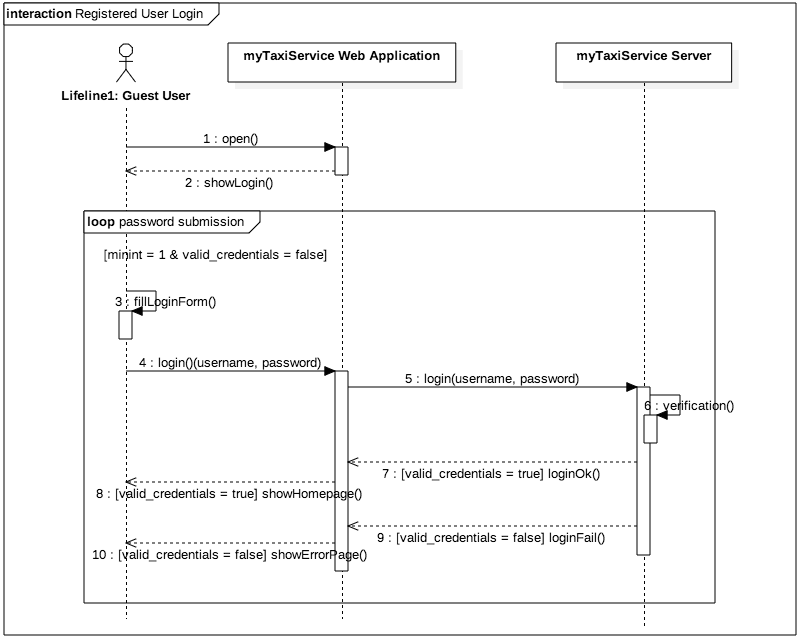
\includegraphics[width=\textwidth, scale=0.5]{IMG/InteractionDiagrams/RegisteredUserLogin.png}
					\caption{Login Interaction Diagram}\label{sec:FigureLogin}
				\end{figure}